\documentclass[12pt]{article}

\usepackage[left=1in, right=1in, top=1in, bottom=1in]{geometry}
\usepackage{amsmath}
\usepackage{amssymb}
\usepackage{bm}
\usepackage{tikz}
\usepackage{mathtools}
\usetikzlibrary{automata,positioning,arrows.meta,calc}
\tikzset{>={Latex[scale=1.5]}}

\begin{document}

\title{CS 3133: Homework 3}
\author{Adam Camilli (aocamilli@wpi.edu)}
\date{\today}
\maketitle

\begin{enumerate}

\item \textbf{5.1} (184) Let M be the DFA defined by \\
  \begin{minipage}{0.5\textwidth}
    \begin{align*}
      &Q = \{q_0,q_1,q_2\} \\   
      &\sum = \{a,b\} \\
      &F = \{q_2\} \\
    \end{align*}
  \end{minipage}
  \begin{minipage}{.5\textwidth}
    \begin{tabular}{c|cc}
      $\delta$ & $a$ & $b$ \\
      \hline
      $q_0$ & $q_0$ & $q_1$ \\
      $q_1$ & $q_2$ & $q_1$ \\
      $q_2$ & $q_2$ & $q_0$ \\
    \end{tabular} \\
  \end{minipage}

  \begin{enumerate}
    \item Give the state diagram of M.
      \begin{center}
        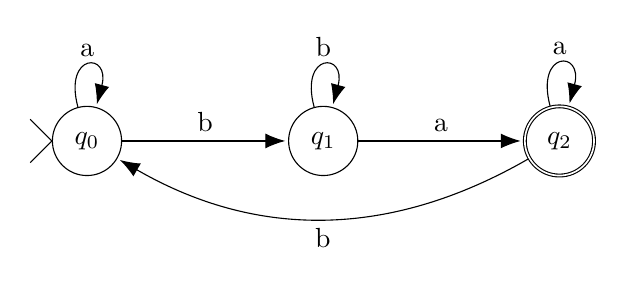
\begin{tikzpicture}[shorten >=1pt, node distance=3cm,auto,]
          \node[state] (q0) {$q_0$}; %initial
          \draw (q0.west) -- ++(-3mm,3mm);
          \draw (q0.west) -- ++(-3mm,-3mm);
          \node[state] (q1) [right of=q0] {$q_1$};
        \node[state,accepting] (q2) [right of=q1] {$q_2$};
        \path[->] (q0) edge [loop above] node {a} ()
                  (q0) edge node {b} (q1)
                  (q1) edge node {a} (q2)
                  (q1) edge [loop above] node {b} (q1)
                  (q2) edge [loop above] node {a} ()
                  (q2) edge [bend left] node {b} (q0);
      \end{tikzpicture}
      \end{center}
    \item Trace the computations of M that process the strings $abaa$, $bbbabb$, $bababa$, and $bbbaa$.\\
      \begin{minipage}[t]{0.22\textwidth}
        \begin{align*}
          &\text{ }[q_0,abaa] \\
          \vdash &\text{ }[q_0,baa] \\
          \vdash &\text{ }[q_1,aa] \\
        \vdash &\text{ }[q_2,a] \\
          \vdash &\text{ }[q_2,\lambda] \text{ } \checkmark \text{ (Accept)} \\
        \end{align*}
      \end{minipage}
      \begin{minipage}[t]{0.22\textwidth}
        \begin{align*}
          &\text{ }[q_0,bbbabb] \\
          \vdash &\text{ }[q_1,bbabb] \\
          \vdash &\text{ }[q_1,babb] \\
          \vdash &\text{ }[q_1,abb] \\
          \vdash &\text{ }[q_2,bb] \\
          \vdash &\text{ }[q_0,b] \\
          \vdash &\text{ }[q_1,b] \\
          \vdash &\text{ }[q_1,\lambda] \text{ } \textbf{X} \text{ (Reject)} \\
        \end{align*}
      \end{minipage}
      \begin{minipage}[t]{0.22\textwidth}
        \begin{align*}
          &\text{ }[q_0,bababa] \\
        \vdash &\text{ }[q_1,ababa] \\
          \vdash &\text{ }[q_2,baba] \\
          \vdash &\text{ }[q_0,aba] \\
          \vdash &\text{ }[q_0,ba] \\
          \vdash &\text{ }[q_1,a] \\
          \vdash &\text{ }[q_2,\lambda] \text{ } \checkmark \text{ (Accept)} \\
        \end{align*}
      \end{minipage}
      \begin{minipage}[t]{0.22\textwidth}
        \begin{align*}
          &\text{ }[q_0,bbbaa] \\
          \vdash &\text{ }[q_1,bbaa] \\
          \vdash &\text{ }[q_1,baa] \\
          \vdash &\text{ }[q_1,aa] \\
          \vdash &\text{ }[q_2,a] \\
          \vdash &\text{ }[q_2,\lambda] \text{ } \text{ } \checkmark \text{ (Accept)} \\
        \end{align*}
      \end{minipage}
  \newpage
\item Which of the strings from part (b) are accepted by M?
  \\ \\  All of them except $bbbabb$.\\
\item Give a regular expression for L(M).
  \[a^{\star}b^+a^+(ba^{\star}b^+a^+)^{\star} \]
  \end{enumerate}

\item \textbf{5.11} (185) Build a DFA that accepts the set of strings over $\{a,b\}$ in which the number of $a$'s is divisible by three. \\ \\
  This set of strings is equivalent to the regular expression $(b^{\star}ab^{\star}ab^{\star}ab^{\star})^{\star}$ which can be modeled in the following state diagram where each state $q_i \in Q$ represents the remainder of current number of $a$'s divided by three (derived from previous state).
\begin{center}
  \begin{tabular}{c|cc}
    $q_i$ & $a$ & $b$ \\
    \hline
    \tikz[baseline]\node[draw,circle,inner sep=1pt]{$q_0$}; & $q_1$ & $q_0$ \\
    $q_1$ & $q_2$ & $q_1$ \\
    $q_2$ & $q_0$ & $q_2$ \\
  \end{tabular}
\end{center}
which corresponds to the state diagram
\begin{center}
  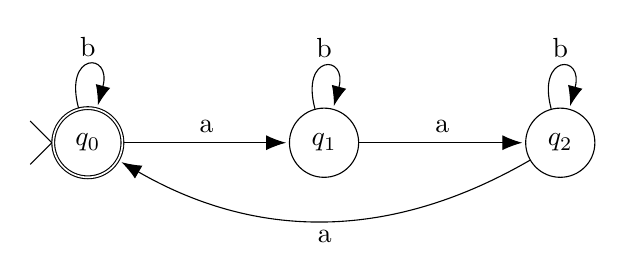
\begin{tikzpicture}[shorten >=1pt, node distance=3cm,auto]
    \node[state,accepting] (q0) {$q_0$}; %initial
    \draw (q0.west) -- ++(-3mm,3mm);
    \draw (q0.west) -- ++(-3mm,-3mm);
    \node[state] (q1) [right of=q0] {$q_1$};
    \node[state] (q2) [right of=q1] {$q_2$};
    \path[->] (q0) edge [loop above] node {b} (0)
              (q0) edge node {a} (q1)
              (q1) edge [loop above] node {b} (q1)
              (q1) edge node {a} (q2)
              (q2) edge [loop above] node {b} (q2)
              (q2) edge [bend left] node {a} (q0);
            \end{tikzpicture}
          \end{center}

\newpage

\item Design a DFA that accepts the language consisting of the set of those strings over $\{a,b,c\}$ in which the number of $a$'s plus the number of $b$'s plus twice the number of $c$'s is divisible by six.
\\ \\ 
The language $L$ that we wish to accept is $L = \{a^l \cup b^m \cup c^n \text{ \big| } (l + m + 2n) \text{ mod } 6 = 0\}$. Designing a regular expression for this language is quite difficult, so it will be more efficient to jump straight to a state table to describe the behavior of a DFA M that accepts this language, with each state $q_i \in Q$ representing the remainder $i$ of dividing the current $(l+m+2n)$ by 6 (derived from previous state). Since $a$ and $b$ affect this value equally, they are grouped together:
\begin{center}
  \begin{tabular}{c|cc}
    $q_i$ & $(a,b)$ & $c$ \\
    \hline
    \tikz[baseline]\node[draw,circle,inner sep=1pt]{$q_0$}; & $q_1$ & $q_2$ \\
    $q_1$ & $q_2$ & $q_3$ \\
    $q_2$ & $q_3$ & $q_4$ \\
    $q_3$ & $q_4$ & $q_5$ \\
    $q_4$ & $q_5$ & $q_0$ \\
    $q_5$ & $q_0$ & $q_1$ \\
  \end{tabular}
\end{center}
From here, we can draw the state diagram:
\begin{center}
  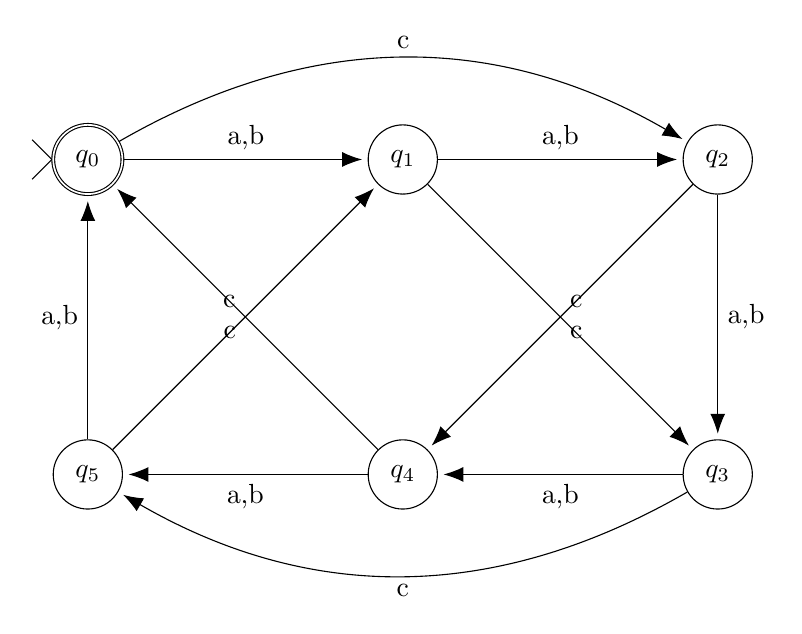
\begin{tikzpicture}[shorten >=2pt, node distance=4cm, auto]
    \node[state,accepting] (q0) {$q_0$};
    \draw (q0.west) -- ++(-3mm,3mm);
    \draw (q0.west) -- ++(-3mm,-3mm);
    \node[state] (q1) [right of=q0] {$q_1$};
    \node[state] (q2) [right of=q1] {$q_2$};
    \node[state] (q3) [below of=q2] {$q_3$};
    \node[state] (q4) [below of=q1] {$q_4$};
    \node[state] (q5) [below of=q0] {$q_5$};
    \path[->] (q0) edge node {a,b} (q1)
              (q0) edge [bend left] node {c} (q2)
              (q1) edge node {a,b} (q2)
              (q1) edge node {c} (q3)
              (q2) edge node {a,b} (q3)
              (q2) edge node [bend right] {c} (q4)
              (q3) edge node {a,b} (q4)
              (q3) edge [bend left] node {c} (q5)
              (q4) edge node {c} (q0)
              (q4) edge node {a,b} (q5)
              (q5) edge node {a,b} (q0)
              (q5) edge node {c} (q1);
            \end{tikzpicture}
          \end{center}
        \newpage  

\item Draw an NFA that accepts the following language over the alphabet ${a,b,c}$:
  \[ \bm{(abc)^{\star}(ab)^{\star}} \]
  Since this language includes $\lambda$, we make the starting state accepting, and simply ensure that from there $\not\exists$ any path to an accepting state that does not go from $a$ to $b$ or from $a$ to $b$ to $c$. Since this is an NFA, we are perfectly fine with only assigning transitions to ``correct'' inputs and allowing ``incorrect'' inputs such as $ac$ or $b$ to cause the automaton to choke and not progress.

\begin{center}
  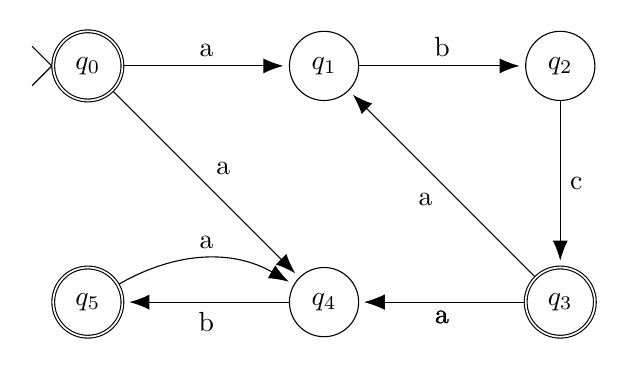
\begin{tikzpicture}[shorten >=2pt, node distance=3cm, auto]
    \node[state,accepting] (q0) {$q_0$}; %initial
    \draw (q0.west) -- ++(-3mm,3mm);
    \draw (q0.west) -- ++(-3mm,-3mm);
    \node[state] (q1) [right of=q0] {$q_1$};
    \node[state] (q2) [right of=q1] {$q_2$};
    \node[state,accepting] (q3) [below of=q2] {$q_3$};
    \node[state] (q4) [left of=q3] {$q_4$};
    \node[state, accepting] (q5) [left of=q4] {$q_5$};
    \path[->] (q0) edge node {a} (q1)
              (q0) edge node {a} (q4)
              (q1) edge node {b} (q2)
              (q2) edge node {c} (q3)
              (q3) edge node {a} (q1)
              (q3) edge node {a} (q4)
              (q3) edge node {a} (q4)
              (q3) edge node {a} (q4)
              (q4) edge node {b} (q5)
              (q5) edge [bend left] node {a} (q4);
            \end{tikzpicture}
          \end{center} 

\newpage

\item \textbf{5.36} (187) Let M be the NFA-$\lambda$
  
  \begin{center}
    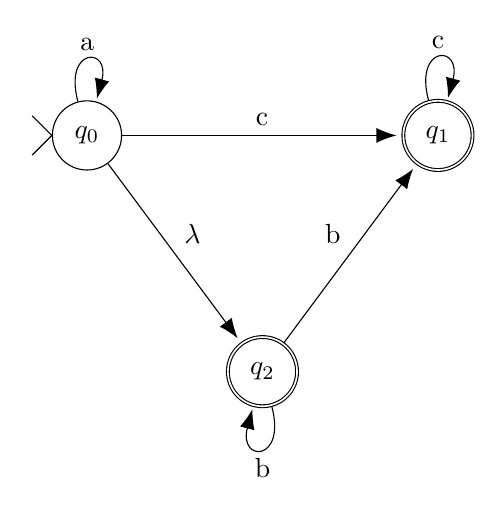
\begin{tikzpicture}[shorten >=2pt, node distance=3cm, auto]
      \node[state] (q0) {$q_0$}; %initial
      \draw (q0.west) -- ++(-3mm,3mm);
      \draw (q0.west) -- ++(-3mm,-3mm);
      \node[state,accepting] (q1) [right=4cm] {$q_1$};
      \node[state,accepting] (q2) [below of=q0] at ($(q0)!0.5!(q1)$) {$q_2$};
      \path[->] (q0) edge [loop above] node {a} (q0)
                (q0) edge node {c} (q1)
                (q0) edge node {$\lambda$} (q2)
                (q1) edge [loop above] node {c} (q1)
                (q2) edge [loop below] node {b} (q2)
                (q2) edge node {b} (q1);
    \end{tikzpicture}      
  \end{center} 
  \begin{enumerate}
    \item Compute $\lambda\text{-}closure(q_i)$ for $i=0,1,2$. \\
      \begin{align*}
        &\lambda\text{-}(q_0) = \{q_0,q_2\} \\
        &\lambda\text{-}(q_1) = \{q_1\} \\
        &\lambda\text{-}(q_2) = \{q_2\}  \\
      \end{align*}
    \item Give the input transition function $t$ for M. \\ \\
      Defining \[ t(q_i, a) = \bigcup_{q_j \in \lambda\text{-}closure(q_i)} \lambda\text{-}closure(\delta(q_j,a))\] we may convert from 
      \begin{center}
        \begin{tabular}{c|cccc}
          $\delta$ & $a$ & $b$ & $c$ & $\lambda$ \\
          \hline
          $q_0$ & $\{q_0\}$ & $\emptyset$ & $\{q_1\}$ & $\{q_2\}$ \\
          $q_1$ & $\emptyset$ & $\emptyset$ & $\{q_1\}$ & $\emptyset$ \\
          $q_2$ & $\emptyset$ & $\{q_2,q_1\}$ & $\emptyset$ & $\emptyset$ \\          
        \end{tabular}
      \end{center}
      
      \hspace{2cm}$\Rightarrow$
      
      \begin{center}
        \begin{tabular}{c|ccc}
          $t$ & $a$ & $b$ & $c$ \\
          \hline
          $q_0$ & $\{q_0,q_2\}$ & $\{q_2,q_1\}$ & $\{q_1\}$ \\
          $q_1$ & $\emptyset$ & $\emptyset$ & $\{q_1\}$ \\
          $q_2$ & $\emptyset$ & $\{q_2,q_1\}$ & $\emptyset$ \\          
        \end{tabular}
      \end{center}

    \item Use Algorithm 5.6.3 to construct a state diagram of a DFA that is equivalent to M. \\
      \begin{enumerate}
        \item Initialize a new set of states Q$'$ as $\lambda\text{-}closure(q_0)$.
          \[ \text{Q}'=\{q_0,q_2\} \]
        \item Begin a transition table with $\sum\{a,b,c\}$ using Q$'$: 
          \begin{center}
            \begin{tabular}{c|ccc}
              $\delta$ & $a$ & $b$ & $c$ \\
              \hline
              $\{q_0,q_2\}$ & $q_0$ & $\{q_2,q_1\}$ & $q_1$ \\
            \end{tabular}
          \end{center} 
        \item Here we see two new states $\{q_1\}, \{q_2,q_1\} \not \in $ Q$'$, so add them to the table: 
          \begin{center}
            \begin{tabular}{c|ccc}
              $\delta$ & $a$ & $b$ & $c$ \\
              \hline
              $\{q_0,q_2\}$ & $\{q_0\}$ & $\{q_2,q_1\}$ & $\{q_1\}$ \\
              $\{q_2,q_1\}$ & $\emptyset$ & $\{q_2,q_1\}$ & $\{q_1\}$ \\
              $\{q_1\}$ & $\emptyset$ & $\emptyset$ & $\{q_1\}$ \\
            \end{tabular}
          \end{center} 
        \item We have no more new states, so now we may draw a DFA, with all invalid inputs going to a ``death state'': \\
        \begin{center}
          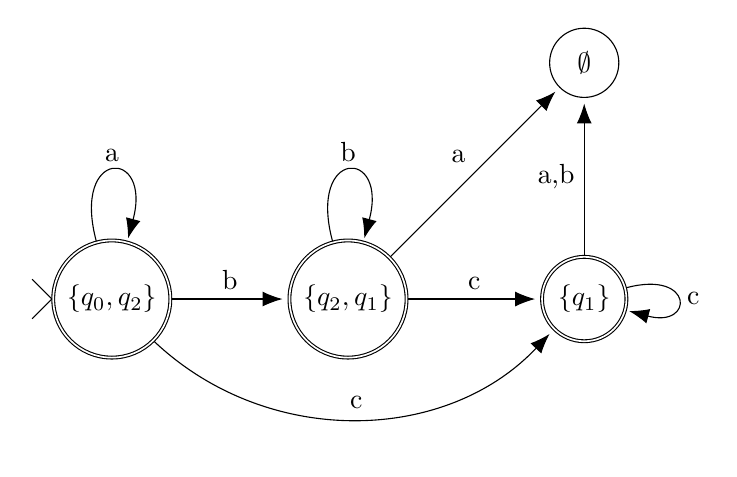
\begin{tikzpicture}[shorten >=2pt, node distance=3cm, auto]
            \node[state,accepting] (q0q2) {$\{q_0,q_2\}$}; %initial
            \draw (q0q2.west) -- ++(-3mm,3mm);
            \draw (q0q2.west) -- ++(-3mm,-3mm);
            \node[state,accepting] (q2q1) [right of=q0q2] {$\{q_2,q_1\}$};
            \node[state,accepting] (q1) [right of=q2q1] {$\{q_1\}$};
            \node[state] (qe) [above of=q1] {$\emptyset$};
            \path[->] (q0q2) edge [loop above] node {a} (q0q2)
                      (q0q2) edge node {b} (q2q1)
                      (q0q2) edge [bend right=45] node {c} (q1)
                      (q2q1) edge [loop above] node {b} (q2q1)
                      (q2q1) edge node {c} (q1)
                      (q2q1) edge node {a} (qe)
                      (q1) edge [loop right] node {c} (q1)
                      (q1) edge node {a,b} (qe);
                    \end{tikzpicture}      
                  \end{center}
                \end{enumerate}
        
    \item Give a regular expression for L(M).
      \[\text{L(M)} = a^{\star}b^{\star}c^{\star} \]
  \end{enumerate}

\end{enumerate}

\end{document}